% Ian Wilkes 
% Artificial Intelligence 600.335
% Assignment 4.
\documentclass[12pt, letterpaper]{article}
\usepackage{amsmath, amsthm, graphicx}


\title{Decision Trees for Classification: \\ An Evolutionary Approach}

\author{Ian Wilkes}

\begin{document}

\maketitle

\begin{abstract}
Classification is one of many extremely important topics within the field of 
artificial intelligence, and is used in many fields from advertising to 
quality control.  As such it is imperative that we be able to provide efficient
and accurate classifiers. One such method for classification is through the use
of decision trees.  This paper will discuss two implementations of decision trees, one using information gain, and another which evolves to learn to classify
sets of data.  Their comparative performance will be discussed, as well as 
ways to optimize each of their individual performance. 


\end{abstract}

\section{Introduction}

\section{Learning Decision Trees}
\subsection{Information-Theoretic Methods}
\subsubsection*{Entropy and Information Gain}
\subsection{Genetic Algorithms}

\subsubsection*{Genetic Algorithms for Decision Trees}

\section{Algorithms and Experimental Methods}

\subsection*{Data Sets}

\section{Results}
\begin{figure}[!htb]
\begin{center}
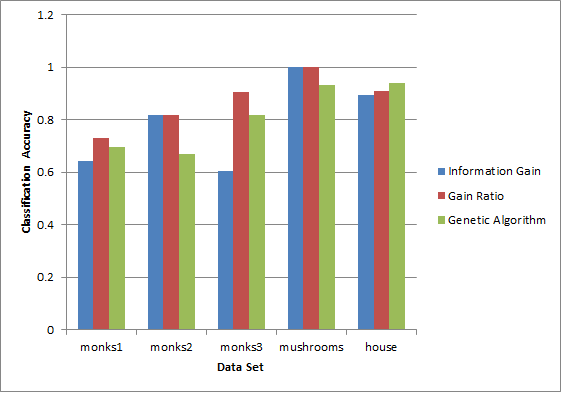
\includegraphics[width=4in]{images/algorithm_comparison_accuracy.png}
\end{center}
\caption{This figure shows the classification accuracy of the information gain
based, gain ratio, and genetic decision trees.  It can be seen that the gain 
ratio based tree seems to perform the best in almost all cases.}
\label{Classification Accuracies of Multiple Decision Trees}
\end{figure}

\begin{figure}[!htb]
\begin{center}
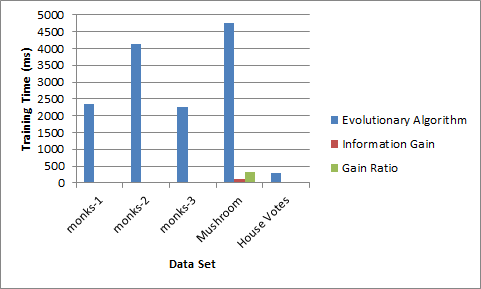
\includegraphics[width=4in]{images/algorithm_comparison_training_time.png}
\end{center}
\caption{This figure shows the required training times of the information gain
based, gain ratio, and genetic decision trees.  It can be seen that the genetic
tree takes much more time than either of the other trees.}
\label{Training Times of Multiple Decision Trees}
\end{figure}

\begin{figure}[!htb]
\begin{center}
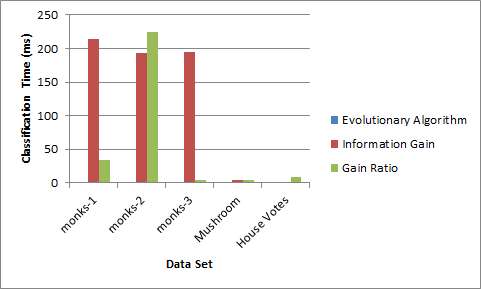
\includegraphics[width=4in]{images/algorithm_comparison_testing_time.png}
\end{center}
\caption{This figure shows the testing time of the information gain
based, gain ratio, and genetic decision trees.  Here, the evolutionary or 
genetic tree takes orders of magnitude less time than the information based
trees.}
\label{Testing Times of Multiple Decision Trees}
\end{figure}


\begin{figure}[!htb]
\begin{center}
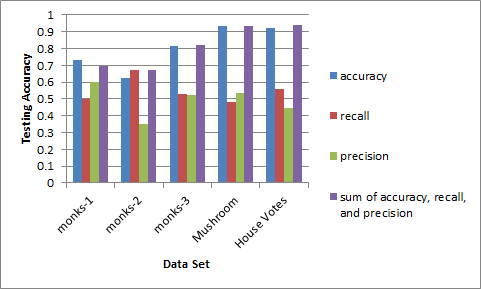
\includegraphics[width=4in]{images/fitness_comparison.png}
\end{center}
\caption{This figure shows the results of using different fitness functions on
the classification accuracy of the genetic tree.}
\label{Classification Accuracies Using Various Fitness Functions}
\end{figure}


\begin{figure}[!htb]
\begin{center}
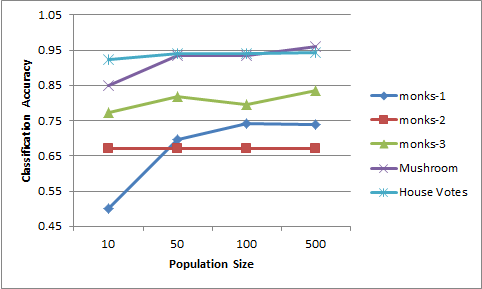
\includegraphics[width=4in]{images/population_comparison.png}
\end{center}
\caption{Here the performance of the genetic algorithm on different data sets
is shown for different population sizes.  For four of the five data sets, the
population must be above 10 individuals to get the best classification accuracy.
}
\label{Testing Times of Multiple Decision Trees}
\end{figure}



\begin{figure}[!htb]
\begin{center}
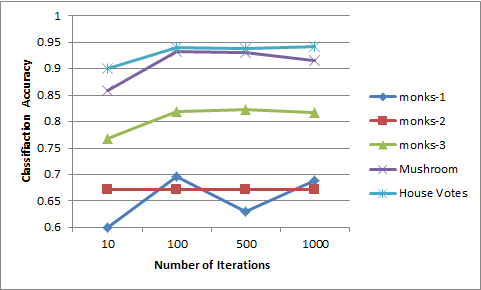
\includegraphics[width=4in]{images/iteration_comparison.png}
\end{center}
\caption{Here the performance of the genetic algorithm on different data sets
is shown for different numbers of training iterations.  For four of the five 
data sets, at least 100 iterations are required to get optimal classification 
accuracies.  
}
\label{Testing Times of Multiple Decision Trees}
\end{figure}


%9
\begin{figure}[!htb]
\begin{center}
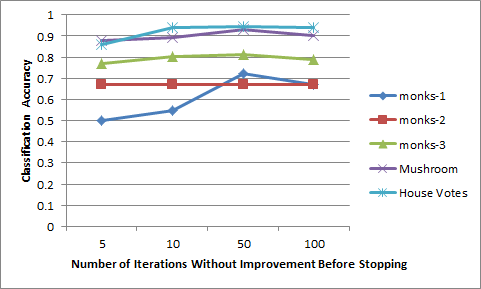
\includegraphics[width=4in]{images/cutoff_accuracy.png}
\end{center}
\caption{This plot shows the effects of the cutoff value on the classification
accuracy of the genetic algorithm for different data sets.  The accuracy seems
to plateau after a certain cutoff value, indicating little effect.
}
\label{Testing Times of Multiple Decision Trees}
\end{figure}

%10
\begin{figure}[!htb]
\begin{center}
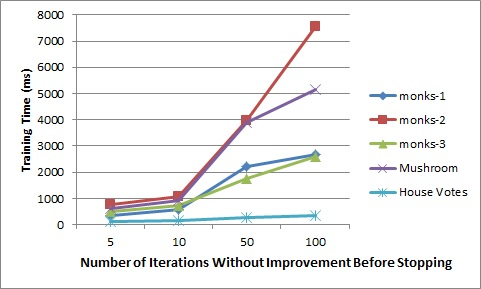
\includegraphics[width=4in]{images/cutoff_time.jpg}
\end{center}
\caption{It can clearly be seen that the time required for training to finish
increases drastically as the cutoff parameter increases for all data sets. 
}
\label{Testing Times of Multiple Decision Trees}
\end{figure}

\begin{table}
\begin{center}
\begin{tabular}{|c||c|cc}
\hline
& col1 & col2 & col3\\
\hline \hline
row1 & a & b & c\\
\hline 
row2 & d & e & f\\
\hline 
row3 & g &   & h\\
 & i & j & k\\
\hline 
\end{tabular}
\end{center}
\caption{This is a caption on the table.  Try to keep your captions short; don't
put multiple paragraphs of text in here.  Put the long version in the Results
section, and reference the table from there.}
\label{sometable}
\end{table}

For all the data shown in this section, the basline genetic algorithm used the 
following parameters which were determined through minimal testing by hand.  
All parameters remain constant, except in the case where they are being
examined one by one.  The mutation and crossover probabilities were 0.01 and 
0.7 respectively.  The population size was 50, and 100 iterations were 
performed.  The default cutoff value was 50.
The standard fitness function used was the sum of the classification accuracy,
recall and precision for each iteration.  Finally, all data presented here is 
the average of five trials for each data point.  

From figure 1 we can see that the performances of the genetic, information
gain and gain ratio based trees are all somewhat comparable.  The gain ratio
tree seems to perform the best of the three in all but the house votes data set.
It drastically out performs the information gain based tree on the monks-3 data
set, whcih is also beaten by the genetic algorithm.

Moving on to figure 2, it is plain to see that the evolutionary algorithm
takes much longer to train than the traditional decision trees, neither of which
ever takes even 500ms to train, while the genetic tree takes almost 5000ms on 
the mushroom data set.

The opposite trend can be seen in the classification times of the testing sets,
which can be observed in figure 3.
The information gain and gain ratio trees take orders of magnitued more time
to classify their data on the monks-1, monks-2, and monks-3 data sets than the
genetic tree.

Figures 4 through 10 show the results from various experiments performed to 
try to optimize the genetic tree shown above. The first of these is figure 4
which shows the effect on classification accuracy of various fitness functions.
It can clearly be seen that by not using the accuracy as one of the components
of the fitness function, the resulting classification accuracy is greatly
reduced, as seen in the cases where recall and precision were used as the 
fitness metrics.

Another parameter which was varied was the population size within the genetic
algorithm based tree.  From figure 5, it can be seen that below a certain 
population threshold the classification performance decreases, yet above that
threshold, an increase in population size does not neccesarily result in 
improved classification performance. The same trend can be seen for the number
of iterations used to train the tree in figure 6. Other than the monks-2 data 
set, all data sets showed a classification accuracy increase by increasing the
number of iterations from 10 to 100.

The effects of mutation and crossover probabilities can be seen in figures 7 
and 8 respectively.  In both cases, the change in the probabilities seem to 
cause different results for the different data sets.  Increasing the mutation
seems to hurt the Mushroom accuracy, while it helps the monks-1 accuracy going
from 0.03 to 0.05.  Similarly for crossover, accuracy is highest for monks-3 
when the crossover probability is 0.9, but this value causes the accuracy for
both the monks-1 and mushroom data sets to decresse significantly.  

Finally, the influence of the cutoff parameter, which stops iteration if no
improvements have been found after a given number of iterations, is shown in
figures 9 and 10. In figure 9, the effect on accuracy can be seen to be minimal
for high values of the cutoff parameter, as the performance for most data sets
stays fairly constant. Figure 10 shows that while the performance may not 
change, the computation time to train the GA increases substantially.    


\section{Discussion}
The discussion section is where you discuss your interpretation of the data you
presented in the results section.  This is where you tell the reader how great
your algorithm is, and how interesting it is that \emph{this} performed better
than \emph{that} on some given data set.  You can also speculate about causes
for interesting behaviors; for example, if you think you might know why it fails
so badly on some particular case, or if you have an insight into why it did well
on another case.  You don't want to be making wild guesses, but as long as you
make it clear that you are not making claims of factual proof, you can go out on
a limb a little.  For example,

\begin{quote}
``In most cases, algorithm A outperforms algorithm B with a significance of
99.8\%.  However, as can be seen from Figure \ref{somefigure}, when applied to
the ``E. E. Smith'' data set, algorithm A does no better than random chance.  It
seems likely that the failure of algorithm A to learn is due to the extremely
sparse distribution of that data set.  Because of algorithm A's heavy reliance
on data being densely sampled from the true underlying distribution, any sparse
data set is likely to show this behavior.''
\end{quote}

Think about the kinds of questions that were posed in the written portions of
homework assignments 1 and 2; these are the kinds of things you want to think
about for your Discussion.

\section{Conclusions}
The conclusion section should be relatively short, and should not be a summary
of your paper.  It should, however, bring up what you learned and what impact
your results have on the rest of the field (and society as a whole, if
applicable, but don't overstate the impact of what you're doing).  You should
conclude, and bring your paper to an end with any parting thoughts that are
appropriate.

Certain types of papers can be ended with a ``Summary'' section instead of a
``Conclusions'' section, in which case you would, in fact, summarize the main
points of your paper.  For this paper, you should write a Conclusions section,
not a Summary.

Conclusion also often contain information about what else you would like
to do.  Sometimes this is a separate subsection, or even a section, entitled
``Future Work.''  The basic idea here is to talk about what the next steps to
take would be.  This is of benefit to others who are interested in your
work and may want to help advance it.  It is also a chance for you to
acknowledge shortcomings in your work; since we never have infinite time to
prepare a paper, there are always more experiments that would have been nice to
include.  If you list them as future work, then it at least makes it clear that
you didn't do those things because you didn't have time, rather than because you
didn't realise that they were important to do.

In your paper, you should include a brief discussion of avenues for possible
future work in your Conclusions section.  It should be tied in with the rest of
your conclusion, and should not be an unrelated section tacked on the end (or
the middle).

% many different styles of bibliography are available; plain is fine for this
% assignment
\bibliographystyle{plain}

% the bibliography command should contain the name of your .bib file, minus the
% extension.
\bibliography{templateBibliography}

% because "document" is an environment, you need to have a closing tag at the
% end of your document.  Anything written after this tag will not be included in
% the generated output.
\end{document}

For example, here is some text that will never show up.
